\documentclass[12pt,letterpaper]{article}

% --- Paquetes ---
\usepackage[T1]{fontenc}
\usepackage[utf8]{inputenc}
\usepackage[spanish,es-noshorthands]{babel}
\usepackage[margin=2.5cm]{geometry}
\usepackage{graphicx}
\usepackage{mathptmx} % Fuente estilo Times New Roman
\usepackage{booktabs}  % Tablas simples con líneas finas
\usepackage{array}
\usepackage{caption}   % Formato de las notas de tabla
\usepackage{float}     % Permite [H] para fijar las tablas
\usepackage{listings}
\usepackage{amsmath}
\usepackage{longtable}  % Tablas que se parten entre páginas

\usepackage[table]{xcolor}  % Colores de celdas

% --- Colores de la tabla M[A, a] ---
\definecolor{celdaazul}{HTML}{DCE6F5}      % Producciones por FIRST
\definecolor{celdaamarilla}{HTML}{FFF2CC}  % Producciones ε por FOLLOW
\newcommand{\fa}[1]{\cellcolor{celdaazul}#1}
\newcommand{\fo}[1]{\cellcolor{celdaamarilla}\textbf{#1}}

% --- Configuración del Índice (TOC) ---
\setcounter{secnumdepth}{0} % Sin numeración de títulos en el texto

% --- Altura de los logos ---
\newcommand{\alturaUNAM}{3.5cm}
\newcommand{\alturaFI}{4.2cm}

% --- Estilo de tablas ---
\newcommand{\cod}[1]{\texttt{#1}} % Texto en monoespaciado
\newcommand{\anchotabla}{0.9\textwidth} % Ancho común de las tablas

% --- Estilo de la nota de tabla ---
\captionsetup[table]{
    labelsep=period,   % "Tabla 1." en lugar de "Tabla 1:"
    justification=centering,
    singlelinecheck=false,
    font=small,
    position=below,
    skip=4pt           % Espacio entre la tabla y su nota
}

\setlength{\intextsep}{6pt} % Espacio arriba/abajo de cada tabla

% --- Nombre de la etiqueta de las tablas en inglés ---
\addto\captionsspanish{\renewcommand{\tablename}{Table}\renewcommand{\figurename}{Figure}\renewcommand{\contentsname}{Table of Contents}}

\begin{document}
% --- Nombre de la etiqueta de las tablas en inglés ---
\addto\captionsspanish{\renewcommand{\tablename}{Table}\renewcommand{\figurename}{Figure}\renewcommand{\contentsname}{Table of Contents}}

\begin{titlepage}
    \centering

    % --- LOGOS AT THE TOP ---
    \begin{minipage}[c]{0.35\textwidth}
        \centering
        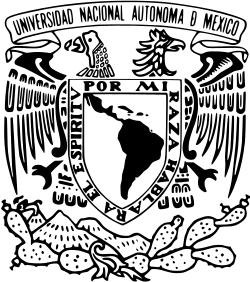
\includegraphics[height=\alturaUNAM]{Escudo-UNAM-escalable.svg.png} % UNAM Logo
    \end{minipage}%
    \hfill
    \begin{minipage}[c]{0.35\textwidth}
        \centering
        
\includegraphics[height=\alturaFI]{EscudoFIVectorizadoNegro2008PPNGx5.png} % FI Logo
    \end{minipage}

    \vspace{1cm}

    % --- UNIVERSITY HEADER BELOW LOGOS ---
    {\Large \textbf{UNIVERSIDAD NACIONAL AUTÓNOMA DE MÉXICO}}\\[0.3cm]
    {\large \textbf{FACULTAD DE INGENIERÍA}}\\[0.3cm]

    \vfill
    \rule{\linewidth}{1.5pt}\\[0.6cm]

    % --- TITLE & SUBTITLE ---
    {\Large \textbf{PARSER AND SYNTAX DIRECTED TRANSLATION}}\\[0.4cm]

    \rule{\linewidth}{1.5pt}
    \vfill

    % --- DETAILS & STUDENT INFO ---
    \begin{flushleft}
        \large
        \textbf{Course:} Compiladores\\[0.2cm]
        \textbf{Group:} 05\\[0.2cm]
        \textbf{Professor:} M.C. René Adrian Dávila Pérez\\[0.2cm]
        \textbf{Student(s):}\\[0.2cm]
        \hspace*{2.8cm} Ambriz Cano Diego Emilio\\[0.2cm]
        \hspace*{2.8cm} Casillas Juárez Camila\\[0.2cm]
        \hspace*{2.8cm} Ferrer Cordero José Manuel\\[0.2cm]
        \hspace*{2.8cm} González Casimiro Juan Carlos\\[0.2cm]
        \hspace*{2.8cm} Vidrio López Mario Alexis\\[0.2cm]
    \end{flushleft}

    \vfill

\end{titlepage}

\newpage
\pagenumbering{arabic} % Comienza la numeración de páginas en 1
\tableofcontents
\newpage

% --- CONTENIDO DEL DOCUMENTO ---

%=====================================================================
\section{Introduction}

In the compilation process, the \textbf{Parser} (or syntactic analyzer) plays a fundamental role. While the previous phase---the \textbf{Lexical Analyzer (Lexer)}---converts the raw input stream of characters into a sequence of classified tokens, the Parser receives these tokens to verify their grammatical structure. Its primary function is to build a hierarchical data structure known as a \textbf{Parse Tree}.\\

Building upon the previous work on the \textit{Lexical Analyzer}, which generated the token sequence required for syntactic analysis, this document details the complete design and implementation of a \textbf{non-recursive Top-Down $\text{LL}(1)$ Parser}. Although various strategies exist for parser construction, this work focuses strictly on the aforementioned deterministic approach.

\section{Top-Down Parsing}

Top-Down Parsing (or Predictive Parsing) is a parsing method in compiler theory that attempts to construct the syntax tree starting from the initial symbol (or root) of the formal grammar downwards, successively applying its production rules to the non-terminal symbols until generating an exact string of terminal symbols matching the source code input.\\

In this project, a non-recursive LL(1) predictive Top-Down parser was chosen. Its classification is Top-Down, non-backtracking, and predictive. The acronym stands for: reads the input from Left to right (L), constructs a Leftmost derivation (L), and decides using 1 symbol of lookahead.\\

The following comparative table presents some of the arguments supporting the construction of the Parser using the LL(1) Top-Down strategy.\\

% ---------------------------------------------------------------------
% TABLA: Top-Down LL(1) vs Bottom-Up
% ---------------------------------------------------------------------
\begin{table}[H]
\centering
\small
\renewcommand{\arraystretch}{1.2}
\begin{tabular}{@{}>{\raggedright\arraybackslash}p{0.20\dimexpr\anchotabla}
                  >{\raggedright\arraybackslash}p{0.36\dimexpr\anchotabla}
                  >{\raggedright\arraybackslash}p{0.38\dimexpr\anchotabla}@{}}
\toprule
\textbf{Criterion} & \textbf{Top-Down LL(1)} & \textbf{Bottom-Up LR(0), SLR(1), LALR(1), CLR(1)} \\
\midrule
Tree construction &
From the root to the leaves &
From the leaves to the root (shift-reduce) \\
\addlinespace
Grammars accepted &
LL(1) grammars, verified through their selection sets and predictive table. &
More grammars, including left recursion. \\
\addlinespace
Compatibility with the grammar &
Yes: it is already LL(1) (Table~\ref{tab:ll1check}) &
Yes, but their main advantage, accepting a wider class of grammars (including left recursion), is not needed here because the grammar is already LL(1). \\
\addlinespace
Table construction &
Directly from FIRST and FOLLOW: $12 \times 17$ &
Requires the collection of item sets and the LR automaton \\
\addlinespace
Trace &
Stack, input, and action. &
Stack of states and symbols, with shifts and reductions \\
\bottomrule
\end{tabular}
\caption{Comparison between Top-Down LL(1) and Bottom-Up parsers.}
\end{table}

LL(1) was chosen because the grammar allows decision-making with a single lookahead token and because the table and execution trace facilitate verifying the procedure. Inherited attributes do not dictate the choice of a top-down parser; in this project, they are evaluated on the complete parse tree after syntactic analysis is completed.\\

Top-down parsing consists of four main components for its execution:
\begin{itemize}
    \item \textbf{Input buffer:} The terminal sequence delivered by the Lexer (Table~\ref{tab:tokens}) followed by \texttt{\$}.
    \item \textbf{Stack:} Initially contains \texttt{\$ Program} (top to the right).
    \item \textbf{Table $M[A, a]$:} The parsing table (Table~\ref{tab:parsetable}).
    \item \textbf{Output:} The sequence of production rules applied, forming the parse tree.
\end{itemize}

\section{Lexer tokens}
From the previous assignment, 'Lexical Analyzer', a token classification was defined for string processing. The Lexer delivers each token as a terminal symbol of a grammar; consequently, the Parser does not process individual characters, only terminal sequences. The token classification is shown in the table below.

% ---------------------------------------------------------------------
% TABLA 1: Token del lexer -> Terminal en la gramática
% ---------------------------------------------------------------------
\begin{table}[H]
\centering
\renewcommand{\arraystretch}{1.2}
\begin{tabular}{@{}p{0.48\dimexpr\anchotabla} p{0.48\dimexpr\anchotabla}@{}}
\toprule
\textbf{Lexer token (TokenType)} & \textbf{Grammar terminal} \\
\midrule
INT, FLOAT, CHAR & \cod{int, float, char} \\
ID & \cod{id} \\
INT\_CONST & \cod{num} \\
FLOAT\_CONST & \cod{real} \\
CHAR\_CONST & \cod{chr} \\
ASSIGN & \cod{=} \\
PLUS, MINUS, STAR, SLASH, PERCENT & \cod{+ - * / \%} \\
LPAREN, RPAREN, SEMI & \cod{( ) ;} \\
STRING & \cod{Str}, outside the grammar \\
Any other (return, ==, true\ldots) & its own lexeme (not in the grammar) \\
\bottomrule
\end{tabular}
\caption{Lexer token and its corresponding terminal in the grammar.}\label{tab:tokens}
\end{table}

As an example of using tokens as terminal symbols in the grammar, the Lexer reads \lstinline|int x = 10;| and delivers five tokens. Each token is translated according to the table, with the end-of-input marker \texttt{\$} appended at the end.

% ---------------------------------------------------------------------
% TABLA 2: Ejemplo de la práctica (int x = 10;)
% ---------------------------------------------------------------------
\begin{table}[H]
\centering
\renewcommand{\arraystretch}{1.2}
\begin{tabular}{@{}p{0.24\dimexpr\anchotabla} p{0.24\dimexpr\anchotabla} p{0.24\dimexpr\anchotabla} p{0.24\dimexpr\anchotabla}@{}}
\toprule
\textbf{Lexeme} & \textbf{Lexer token} & \textbf{Terminal} & \textbf{Line} \\
\midrule
\cod{int} & INT & \cod{int} & 1 \\
\cod{x} & ID & \cod{id} & 1 \\
\cod{=} & ASSIGN & \cod{=} & 1 \\
\cod{10} & INT\_CONST & \cod{num} & 1 \\
\cod{;} & SEMI & \cod{;} & 1 \\
(end) & --- & \cod{\$} & 1 \\
\bottomrule
\end{tabular}
\caption{Token example for \texttt{int x = 10;}}
\end{table}

The parser input is then \texttt{int id = num ; \$}. Each input symbol retains its corresponding terminal, lexeme, and line from the original token. The parser makes decisions based on the terminal and uses the remaining data for attributes and diagnostics, as error messages require them (e.g., \texttt{missing ';' after '10', error in line 1}).\\

The specifications of this project require that the productions match the input tokens; therefore, no terminals were created beyond those already produced by the Lexer: each terminal of the grammar corresponds to a \texttt{TokenType} from the Lexer's 45-type catalog, and Table~\ref{tab:tokens} gives the mapping between the \texttt{TokenType} names and the terminal names used in the grammar (e.g., \texttt{INT\_CONST} is written as \texttt{num}).\\

\texttt{"num"}, \texttt{"real"}, and \texttt{"chr"} are separated because the SDT requires the type of each constant. This separation allows directly associating each terminal with its type. It would also be possible to use a common terminal and query the original \texttt{TokenType}, but three terminals were chosen to simplify the semantic rules.\\

\texttt{"return"} arrives as the \texttt{return} terminal, and the Parser reports it as unexpected without needing a special rule: the lexer recognizes it, but it does not belong to the language of this grammar.\\

The lexer retains the recovery mechanism defined in the first stage and can continue to locate multiple errors. However, if it returns any lexical error, the driver bypasses the parser and semantic evaluation. The recovered tokens can be displayed for diagnostics, but they do not allow certifying the validity of the original text.

\section{Parser and SDT}
Below is the context-free grammar for programs consisting of declarations and assignments with arithmetic expressions, built from the proposed grammar of the ``Lexical Analyzer'' submission.\\

% ---------------------------------------------------------------------
% TABLA 3: Gramática G1 del lexer
% ---------------------------------------------------------------------
\begin{table}[H]
\centering
\renewcommand{\arraystretch}{1.2}
\begin{tabular}{@{}p{0.20\dimexpr\anchotabla} p{0.08\dimexpr\anchotabla} p{0.68\dimexpr\anchotabla}@{}}
\toprule
\textbf{Non-terminal} & & \textbf{Productions} \\
\midrule
\cod{Decl}  & $\rightarrow$ & \cod{Type id Decl'} \\
\cod{Decl'} & $\rightarrow$ & \cod{;} $\mid$ \cod{= Value ;} \\
\cod{Type}  & $\rightarrow$ & \cod{int} $\mid$ \cod{float} $\mid$ \cod{char} \\
\cod{Value} & $\rightarrow$ & \cod{num} $\mid$ \cod{id} \\
\bottomrule
\end{tabular}
\caption{Grammar G1 from the Lexer assignment.}
\end{table}

The previous grammar is LL(1), and its terminals are tokens; however, this grammar only accepts a single declaration and a simple value, meaning it does not allow expressions such as \texttt{int y = x * 2;} nor sequences of multiple statements. Below is the generalized grammar for this project.

% ---------------------------------------------------------------------
% TABLA: Gramática completa (27 producciones)
% ---------------------------------------------------------------------
\begin{table}[H]
\centering
\renewcommand{\arraystretch}{1.1}
\begin{tabular}{@{}p{0.08\dimexpr\anchotabla} p{0.20\dimexpr\anchotabla} p{0.08\dimexpr\anchotabla} p{0.60\dimexpr\anchotabla}@{}}
\toprule
\textbf{\#} & \textbf{Non-terminal} & & \textbf{Production} \\
\midrule
1  & \cod{Program}  & $\rightarrow$ & \cod{Stmt StmtList} \\
2  & \cod{StmtList} & $\rightarrow$ & \cod{Stmt StmtList} \\
3  & \cod{StmtList} & $\rightarrow$ & $\varepsilon$ \\
4  & \cod{Stmt}     & $\rightarrow$ & \cod{Decl} \\
5  & \cod{Stmt}     & $\rightarrow$ & \cod{Assign} \\
6  & \cod{Decl}     & $\rightarrow$ & \cod{Type id Decl'} \\
7  & \cod{Decl'}    & $\rightarrow$ & \cod{;} \\
8  & \cod{Decl'}    & $\rightarrow$ & \cod{= Expr ;} \\
9  & \cod{Assign}   & $\rightarrow$ & \cod{id = Expr ;} \\
10 & \cod{Type}     & $\rightarrow$ & \cod{int} \\
11 & \cod{Type}     & $\rightarrow$ & \cod{float} \\
12 & \cod{Type}     & $\rightarrow$ & \cod{char} \\
13 & \cod{Expr}     & $\rightarrow$ & \cod{Term Expr'} \\
14 & \cod{Expr'}    & $\rightarrow$ & \cod{+ Term Expr'} \\
15 & \cod{Expr'}    & $\rightarrow$ & \cod{- Term Expr'} \\
16 & \cod{Expr'}    & $\rightarrow$ & $\varepsilon$ \\
17 & \cod{Term}     & $\rightarrow$ & \cod{Factor Term'} \\
18 & \cod{Term'}    & $\rightarrow$ & \cod{* Factor Term'} \\
19 & \cod{Term'}    & $\rightarrow$ & \cod{/ Factor Term'} \\
20 & \cod{Term'}    & $\rightarrow$ & \cod{\% Factor Term'} \\
21 & \cod{Term'}    & $\rightarrow$ & $\varepsilon$ \\
22 & \cod{Factor}   & $\rightarrow$ & \cod{( Expr )} \\
23 & \cod{Factor}   & $\rightarrow$ & \cod{- Factor} \\
24 & \cod{Factor}   & $\rightarrow$ & \cod{id} \\
25 & \cod{Factor}   & $\rightarrow$ & \cod{num} \\
26 & \cod{Factor}   & $\rightarrow$ & \cod{real} \\
27 & \cod{Factor}   & $\rightarrow$ & \cod{chr} \\
\bottomrule
\end{tabular}
\caption{Complete grammar of the project (27 productions).}
\end{table}

The previous grammar was constructed from the following context-free grammar without left recursion.
\newpage

% ---------------------------------------------------------------------
% TABLA 4: Gramática de expresiones sin recursión por la izquierda
% ---------------------------------------------------------------------
\begin{table}[H]
\centering
\renewcommand{\arraystretch}{1.2}
\begin{tabular}{@{}p{0.20\dimexpr\anchotabla} p{0.08\dimexpr\anchotabla} p{0.68\dimexpr\anchotabla}@{}}
\toprule
\textbf{Non-terminal} & & \textbf{Productions} \\
\midrule
\cod{E}  & $\rightarrow$ & \cod{T E'} \\
\cod{E'} & $\rightarrow$ & \cod{+ T E'} $\mid$ $\varepsilon$ \\
\cod{T}  & $\rightarrow$ & \cod{F T'} \\
\cod{T'} & $\rightarrow$ & \cod{* F T'} $\mid$ $\varepsilon$ \\
\cod{F}  & $\rightarrow$ & \cod{id} $\mid$ \cod{( E )} \\
\bottomrule
\end{tabular}
\caption{Expression grammar without left recursion.}
\end{table}

The previous grammar was proposed during the theoretical sessions of the Compilers course; the grammar was implemented using clearer names (\texttt{Expr}, \texttt{Expr'}, \texttt{Term}, \texttt{Term'}, \texttt{Factor}), and the operators \texttt{-}, \texttt{/}, and \texttt{\%} were added, along with the constants \texttt{num}, \texttt{real}, and \texttt{chr} as factors. \texttt{Value} was replaced by \texttt{Expr}; thus, a declaration now accepts any expression.\\

To support programs containing sequence structures, the productions \texttt{Program} $\rightarrow$ \texttt{Stmt StmtList} and \texttt{StmtList} $\rightarrow$ \texttt{Stmt StmtList} $\mid$ $\varepsilon$ were introduced. This structural design allows the parsing of one or more statements while intentionally rejecting empty inputs. Additionally, statements must be strictly terminated by semicolons (\texttt{;}) rather than line breaks. Furthermore, the inclusion of \texttt{Stmt} $\rightarrow$ \texttt{Decl} $\mid$ \texttt{Assign} alongside \texttt{Assign} $\rightarrow$ \texttt{id = Expr ;} enables the usage of variables after their initial declaration (e.g., \texttt{x = y;}), providing the explicit structure required for the Syntax-Directed Translation (SDT) phase to perform semantic checks.\\

The production \texttt{Factor} $\rightarrow$ \texttt{- Factor} was incorporated into the grammar to allow negative literal constants and expressions, such as \texttt{-5} or \texttt{-x}. In alignment with the lexical analyzer design, constants are treated as unsigned at the lexer level---ensuring expressions like \texttt{a-1} are correctly tokenized as \texttt{a}, \texttt{-}, and \texttt{1}---leaving sign resolution entirely to the parser. While the lexer is capable of recognizing both positive and negative signs, this grammar version intentionally includes only the unary minus; expressions containing a unary plus (such as \texttt{+1}) are not recognized by the defined language rules.\\

Finally, the resulting context-free grammar is formally defined by the tuple $G = (N, T, P, S)$. The set of non-terminals $N$ consists of 12 symbols: \texttt{Program}, \texttt{StmtList}, \texttt{Stmt}, \texttt{Decl}, \texttt{Decl'}, \texttt{Assign}, \texttt{Type}, \texttt{Expr}, \texttt{Expr'}, \texttt{Term}, \texttt{Term'}, and \texttt{Factor}. The set of terminals $T$ contains 16 symbols: \texttt{int}, \texttt{float}, \texttt{char}, \texttt{id}, \texttt{num}, \texttt{real}, \texttt{chr}, \texttt{=}, \texttt{+}, \texttt{-}, \texttt{*}, \texttt{/}, \texttt{\%}, \texttt{(}, \texttt{)}, and \texttt{;}. Lastly, \texttt{Program} is designated as the start symbol $S$ of the grammar.\\
\newpage

\subsection{Verify. Leftmost derivation}

The following table shows the leftmost derivation process for the string \texttt{int id = num;}, always replacing the leftmost non-terminal. The number in parentheses indicates the production used.

% ---------------------------------------------------------------------
% TABLA: Derivación por la izquierda de int x = 10;
% ---------------------------------------------------------------------
\begin{table}[H]
\centering
\renewcommand{\arraystretch}{1.1}
\begin{tabular}{@{}p{0.10\dimexpr\anchotabla} p{0.08\dimexpr\anchotabla} p{0.78\dimexpr\anchotabla}@{}}
\toprule
\textbf{Step} & \textbf{Rule} & \textbf{Sentential form} \\
\midrule
      & ---  & \cod{Program} \\
$\Rightarrow$ & (1)  & \cod{Stmt StmtList} \\
$\Rightarrow$ & (4)  & \cod{Decl StmtList} \\
$\Rightarrow$ & (6)  & \cod{Type id Decl' StmtList} \\
$\Rightarrow$ & (10) & \cod{int id Decl' StmtList} \\
$\Rightarrow$ & (8)  & \cod{int id = Expr ; StmtList} \\
$\Rightarrow$ & (13) & \cod{int id = Term Expr' ; StmtList} \\
$\Rightarrow$ & (17) & \cod{int id = Factor Term' Expr' ; StmtList} \\
$\Rightarrow$ & (25) & \cod{int id = num Term' Expr' ; StmtList} \\
$\Rightarrow$ & (21) & \cod{int id = num Expr' ; StmtList} \\
$\Rightarrow$ & (16) & \cod{int id = num ; StmtList} \\
$\Rightarrow$ & (3)  & \cod{int id = num ;} \\
\bottomrule
\end{tabular}
\caption{Leftmost derivation of \texttt{int x = 10;}.}\label{tab:derivation}
\end{table}

The grammar covers the practice example and enough for the SDT to have something to verify (types, declarations, assignments), without adding unrequested statements (such as \texttt{if} or \texttt{while}) that would make the design harder to defend. The language uses a single global scope. It does not include functions, blocks, arrays, function calls, strings, or booleans. Tokens recognized by the lexer for those constructs are rejected at this stage.

\section{Verification of the Grammar for Top-Down Parsing}
To use the chosen LL(1) predictive parser, the absence of left recursion, factoring, and alternative selection were reviewed. The initial reviews help prepare the grammar, but the definitive check is performed through FIRST, FOLLOW, and the absence of conflicts in the predictive table.
\subsection{Unambiguous}

A grammar is ambiguous if any string has two distinct parse trees. The typical source of ambiguity in expressions is a production like $E \rightarrow E + E \mid E * E$, which allows grouping $a + b * c$ in two different ways.\\

Here, that cannot happen: each precedence level is a separate non-terminal. Addition can only appear in \texttt{Expr'}, and multiplication only in \texttt{Term'}. For $a + b * c$, the only way to derive the $*$ is within the \texttt{Term} following the $+$, so there is only one possible tree. The same applies to statements: each one begins with a type (declaration) or with \texttt{id} (assignment) and ends with \texttt{;}.
\newpage

\subsection{Without left recursion}
Left recursion occurs when a non-terminal can derive a sequence starting with itself ($A \Rightarrow^+ A \alpha$). A top-down parser would enter an infinite loop: to expand $A$, it would have to expand $A$ again without consuming input.\\

There is no direct or indirect left recursion. By following the non-terminals that can appear at the start of a production, dependencies move towards \texttt{Type}, \texttt{Assign}, or \texttt{Factor}, whose alternatives begin with terminals; no cycle is formed that would allow returning to the initial non-terminal without consuming input.

\subsection{Left factoring}
Left factoring is needed when two alternatives of the same non-terminal begin with the same prefix, for example $A \rightarrow a\,b \mid a\,c$: with a single lookahead token, the parser could not decide which alternative to apply. In this grammar, that situation was already resolved in the design: the declaration prefix \texttt{Type id} is shared by declarations with and without an initializer, so it was factored out into \texttt{Decl} $\rightarrow$ \texttt{Type id Decl'}, leaving the two alternatives of \texttt{Decl'} to begin with different terminals (\texttt{;} and \texttt{=}). In every other non-terminal, the alternatives begin with different terminals, as shown in Table~\ref{tab:ll1check}, so no further factoring is required.

\subsection{Condition (LL1)}

For each production $A \rightarrow \alpha$, its select set is obtained as follows:
$$\text{SELECT}(A \rightarrow \alpha) = \text{FIRST}(\alpha) - \{\varepsilon\}$$

If $\alpha$ can derive $\varepsilon$, $\text{FOLLOW}(A)$ is also included.

A grammar is LL(1) if the select sets of the different alternatives for the same non-terminal are disjoint.

% ---------------------------------------------------------------------
% TABLA: Verificación de la condición LL(1) por no terminal
% ---------------------------------------------------------------------
\begin{table}[H]
\centering
\small
\renewcommand{\arraystretch}{1.1}
\newcommand{\cc}{\raggedright\arraybackslash}
\begin{tabular}{@{}>{\cc}p{0.12\dimexpr\anchotabla}
                  >{\cc}p{0.40\dimexpr\anchotabla}
                  >{\cc}p{0.11\dimexpr\anchotabla}
                  >{\cc}p{0.23\dimexpr\anchotabla}
                  >{\cc}p{0.10\dimexpr\anchotabla}@{}}
\toprule
\textbf{Non-terminal} & \textbf{Alternatives and their FIRST} & \textbf{Disjoint FIRST} & \textbf{If an alternative derives $\varepsilon$} & \textbf{LL(1)} \\
\midrule
\cod{StmtList} &
(2) StmtList $\rightarrow$ Stmt StmtList: $\{$ int, float, char, id $\}$ \newline
(3) StmtList $\rightarrow$ $\varepsilon$: $\{$ $\varepsilon$ $\}$ &
yes &
FOLLOW = $\{$ \$ $\}$ \newline intersection: $\emptyset$ &
\textbf{holds} \\
\addlinespace
\cod{Stmt} &
(4) Stmt $\rightarrow$ Decl: $\{$ int, float, char $\}$ \newline
(5) Stmt $\rightarrow$ Assign: $\{$ id $\}$ &
yes &
not applicable &
\textbf{holds} \\
\addlinespace
\cod{Decl'} &
(7) Decl' $\rightarrow$ ;: $\{$ ; $\}$ \newline
(8) Decl' $\rightarrow$ = Expr ;: $\{$ = $\}$ &
yes &
not applicable &
\textbf{holds} \\
\addlinespace
\cod{Type} &
(10) Type $\rightarrow$ int: $\{$ int $\}$ \newline
(11) Type $\rightarrow$ float: $\{$ float $\}$ \newline
(12) Type $\rightarrow$ char: $\{$ char $\}$ &
yes &
not applicable &
\textbf{holds} \\
\addlinespace
\cod{Expr'} &
(14) Expr' $\rightarrow$ + Term Expr': $\{$ + $\}$ \newline
(15) Expr' $\rightarrow$ - Term Expr': $\{$ - $\}$ \newline
(16) Expr' $\rightarrow$ $\varepsilon$: $\{$ $\varepsilon$ $\}$ &
yes &
FOLLOW = $\{$ ), ; $\}$ \newline intersection: $\emptyset$ &
\textbf{holds} \\
\addlinespace
\cod{Term'} &
(18) Term' $\rightarrow$ * Factor Term': $\{$ * $\}$ \newline
(19) Term' $\rightarrow$ / Factor Term': $\{$ / $\}$ \newline
(20) Term' $\rightarrow$ \% Factor Term': $\{$ \% $\}$ \newline
(21) Term' $\rightarrow$ $\varepsilon$: $\{$ $\varepsilon$ $\}$ &
yes &
FOLLOW = $\{$ +, -, ), ; $\}$ \newline intersection: $\emptyset$ &
\textbf{holds} \\
\addlinespace
\cod{Factor} &
(22) Factor $\rightarrow$ ( Expr ): $\{$ ( $\}$ \newline
(23) Factor $\rightarrow$ - Factor: $\{$ - $\}$ \newline
(24) Factor $\rightarrow$ id: $\{$ id $\}$ \newline
(25) Factor $\rightarrow$ num: $\{$ num $\}$ \newline
(26) Factor $\rightarrow$ real: $\{$ real $\}$ \newline
(27) Factor $\rightarrow$ chr: $\{$ chr $\}$ &
yes &
not applicable &
\textbf{holds} \\
\bottomrule
\end{tabular}
\caption{LL(1) condition check for each non-terminal.}\label{tab:ll1check}
\end{table}

All seven non-terminals listed in Table~\ref{tab:ll1check} satisfy the condition. The other five (\texttt{Program}, \texttt{Decl}, \texttt{Assign}, \texttt{Expr}, and \texttt{Term}) have a single production, so they satisfy it trivially. Therefore, the grammar is LL(1).

\section{First}
For each non-terminal $A$, $\text{FIRST}(A)$ was calculated: the set of terminals with which a string derived from $A$ can start, plus $\varepsilon$ if $A$ can derive the empty string. The LL(1) table uses $\text{FIRST}$ to decide which production to apply.

\begin{enumerate}
    \item If $X$ is a terminal, $\text{FIRST}(X) = \{ X \}$.
    \item If there is a production $X \rightarrow \varepsilon$, then $\varepsilon$ is in $\text{FIRST}(X)$.
    \item If $X \rightarrow Y_1 Y_2 \dots Y_k$, $\text{FIRST}(Y_1)$ without $\varepsilon$ is added. If $Y_1$ can derive $\varepsilon$, then $\text{FIRST}(Y_2)$ without $\varepsilon$ is also added, and so on. If all $Y_i$ can derive $\varepsilon$, $\varepsilon$ is added.
\end{enumerate}

% ---------------------------------------------------------------------
% TABLA: Cálculo de FIRST por no terminal
% ---------------------------------------------------------------------
\begin{table}[H]
\centering
\renewcommand{\arraystretch}{1.2}
\begin{tabular}{@{}p{0.30\dimexpr\anchotabla} p{0.66\dimexpr\anchotabla}@{}}
\toprule
\textbf{Non-terminal} & \textbf{FIRST} \\
\midrule
\cod{Factor}   & $\{$ id, num, real, chr, -, ( $\}$ \\
\cod{Term'}    & $\{$ *, /, \%, $\varepsilon$ $\}$ \\
\cod{Term}     & $\{$ id, num, real, chr, -, ( $\}$ \\
\cod{Expr'}    & $\{$ +, -, $\varepsilon$ $\}$ \\
\cod{Expr}     & $\{$ id, num, real, chr, -, ( $\}$ \\
\cod{Type}     & $\{$ int, float, char $\}$ \\
\cod{Decl'}    & $\{$ =, ; $\}$ \\
\cod{Decl}     & $\{$ int, float, char $\}$ \\
\cod{Assign}   & $\{$ id $\}$ \\
\cod{Stmt}     & $\{$ int, float, char, id $\}$ \\
\cod{StmtList} & $\{$ int, float, char, id, $\varepsilon$ $\}$ \\
\cod{Program}  & $\{$ int, float, char, id $\}$ \\
\bottomrule
\end{tabular}
\caption{FIRST set of each non-terminal.}
\end{table}

\section{Follow}

For each non-terminal $A$, $\text{FOLLOW}(A)$ was computed: the set of terminals that can appear immediately after $A$ in some sentential form. The LL(1) table uses $\text{FOLLOW}$ for $\varepsilon$-productions: when $A$ can derive $\varepsilon$, the Parser needs to know which tokens may come after $A$ in order to decide whether to apply that production.

\begin{enumerate}
    \item \texttt{\$} is in $\text{FOLLOW}$ of the start symbol.
    \item If a terminal comes after $A$, that terminal is added to $\text{FOLLOW}(A)$.
    \item If a non-terminal $B$ comes after $A$, $\text{FIRST}(B)$ without $\varepsilon$ is added.
    \item If $A$ is at the end of the right-hand side, or everything that follows it can derive $\varepsilon$, the $\text{FOLLOW}$ of the left-hand side is added.
\end{enumerate}

% ---------------------------------------------------------------------
% TABLA: Cálculo de FOLLOW (dónde aparece cada no terminal)
% ---------------------------------------------------------------------
\begin{table}[H]
\centering
\small
\renewcommand{\arraystretch}{1.1}
\begin{tabular}{@{}p{0.20\dimexpr\anchotabla} p{0.15\dimexpr\anchotabla} p{0.61\dimexpr\anchotabla}@{}}
\toprule
\textbf{Non-terminal} & \textbf{Rule} & \textbf{Contributes to FOLLOW} \\
\midrule
\cod{Program}  & 1     & $\{$ \$ $\}$ \\
\addlinespace
\cod{StmtList} & 3     & $\{$ \$ $\}$ \\
               & 3     & $\{$ \$ $\}$ \\
\addlinespace
\cod{Stmt}     & 2 and 3 & $\{$ int, float, char, id, \$ $\}$ \\
               & 2 and 3 & $\{$ int, float, char, id, \$ $\}$ \\
\addlinespace
\cod{Decl}     & 3     & $\{$ int, float, char, id, \$ $\}$ \\
\addlinespace
\cod{Decl'}    & 3     & $\{$ int, float, char, id, \$ $\}$ \\
\addlinespace
\cod{Assign}   & 3     & $\{$ int, float, char, id, \$ $\}$ \\
\addlinespace
\cod{Type}     & 1     & $\{$ id $\}$ \\
\addlinespace
\cod{Expr}     & 1     & $\{$ ; $\}$ \\
               & 1     & $\{$ ; $\}$ \\
               & 1     & $\{$ ) $\}$ \\
\addlinespace
\cod{Expr'}    & 3     & $\{$ ), ; $\}$ \\
               & 3     & $\{$ ), ; $\}$ \\
               & 3     & $\{$ ), ; $\}$ \\
\addlinespace
\cod{Term}     & 2 and 3 & $\{$ +, -, ), ; $\}$ \\
               & 2 and 3 & $\{$ +, -, ), ; $\}$ \\
               & 2 and 3 & $\{$ +, -, ), ; $\}$ \\
\addlinespace
\cod{Term'}    & 3     & $\{$ +, -, ), ; $\}$ \\
               & 3     & $\{$ +, -, ), ; $\}$ \\
               & 3     & $\{$ +, -, ), ; $\}$ \\
               & 3     & $\{$ +, -, ), ; $\}$ \\
\addlinespace
\cod{Factor}   & 2 and 3 & $\{$ +, -, *, /, \%, ), ; $\}$ \\
               & 2 and 3 & $\{$ +, -, *, /, \%, ), ; $\}$ \\
               & 2 and 3 & $\{$ +, -, *, /, \%, ), ; $\}$ \\
               & 2 and 3 & $\{$ +, -, *, /, \%, ), ; $\}$ \\
               & 3     & $\{$ +, -, *, /, \%, ), ; $\}$ \\
\bottomrule
\end{tabular}
\caption{FOLLOW contributions for each occurrence of a non-terminal.}
\end{table}

To compute $\text{FOLLOW}(A)$, each occurrence of $A$ on the right-hand side of a production is located, and the rule corresponding to what follows it is applied.

\section{First and Follow Summary}
% ---------------------------------------------------------------------
% TABLA: Resultado FIRST y FOLLOW de los 12 no terminales
% ---------------------------------------------------------------------
\begin{table}[H]
\centering
\renewcommand{\arraystretch}{1.2}
\begin{tabular}{@{}p{0.20\dimexpr\anchotabla} p{0.38\dimexpr\anchotabla} p{0.38\dimexpr\anchotabla}@{}}
\toprule
\textbf{Non-terminal} & \textbf{FIRST} & \textbf{FOLLOW} \\
\midrule
\cod{Program}  & $\{$ int, float, char, id $\}$       & $\{$ \$ $\}$ \\
\cod{StmtList} & $\{$ int, float, char, id, $\varepsilon$ $\}$ & $\{$ \$ $\}$ \\
\cod{Stmt}     & $\{$ int, float, char, id $\}$       & $\{$ int, float, char, id, \$ $\}$ \\
\cod{Decl}     & $\{$ int, float, char $\}$           & $\{$ int, float, char, id, \$ $\}$ \\
\cod{Decl'}    & $\{$ =, ; $\}$                       & $\{$ int, float, char, id, \$ $\}$ \\
\cod{Assign}   & $\{$ id $\}$                         & $\{$ int, float, char, id, \$ $\}$ \\
\cod{Type}     & $\{$ int, float, char $\}$           & $\{$ id $\}$ \\
\cod{Expr}     & $\{$ id, num, real, chr, -, ( $\}$   & $\{$ ), ; $\}$ \\
\cod{Expr'}    & $\{$ +, -, $\varepsilon$ $\}$        & $\{$ ), ; $\}$ \\
\cod{Term}     & $\{$ id, num, real, chr, -, ( $\}$   & $\{$ +, -, ), ; $\}$ \\
\cod{Term'}    & $\{$ *, /, \%, $\varepsilon$ $\}$    & $\{$ +, -, ), ; $\}$ \\
\cod{Factor}   & $\{$ id, num, real, chr, -, ( $\}$   & $\{$ +, -, *, /, \%, ), ; $\}$ \\
\bottomrule
\end{tabular}
\caption{FIRST and FOLLOW sets of the 12 non-terminals.}
\end{table}

\section{Parse table}
The parsing table $M[A, a]$ was constructed: one row per non-terminal (the symbol at the top of the stack), one column per terminal (the current token), and, in each cell, the production that the parser must apply. An empty cell indicates a syntax error.\\

The rules for constructing the table are as follows.\\

For each production $A \rightarrow \alpha$:
\begin{enumerate}
    \item \textbf{$\varepsilon$-productions go under $\text{FOLLOW}$}. If $\alpha$ can derive $\varepsilon$, the production is placed in $M[A, b]$ for each terminal $b$ in $\text{FOLLOW}(A)$.
    \item \textbf{The remaining productions go under $\text{FIRST}$}. The production is placed in $M[A, a]$ for each terminal $a$ in $\text{FIRST}(\alpha)$.
\end{enumerate}

% ---------------------------------------------------------------------
% TABLA: Colocación de cada producción (27 producciones)
% ---------------------------------------------------------------------
\begin{table}[H]
\centering
\small
\setlength{\tabcolsep}{3pt}
\renewcommand{\arraystretch}{1.1}
\begin{tabular}{@{}>{\raggedright\arraybackslash}p{0.05\dimexpr\anchotabla}
                  >{\raggedright\arraybackslash}p{0.23\dimexpr\anchotabla}
                  >{\raggedright\arraybackslash}p{0.23\dimexpr\anchotabla}
                  >{\raggedright\arraybackslash}p{0.09\dimexpr\anchotabla}
                  >{\raggedright\arraybackslash}p{0.18\dimexpr\anchotabla}
                  >{\raggedright\arraybackslash}p{0.14\dimexpr\anchotabla}@{}}
\toprule
\textbf{\#} & \textbf{Production} & \textbf{FIRST($\alpha$)} & \textbf{$\alpha \Rightarrow^{*} \varepsilon$} & \textbf{Columns by FIRST (rule 2)} & \textbf{Columns by FOLLOW (rule 1)} \\
\midrule
1  & \cod{Program $\rightarrow$ Stmt StmtList}  & $\{$ int, float, char, id $\}$       & no  & \cod{int float char id}        & --- \\
2  & \cod{StmtList $\rightarrow$ Stmt StmtList} & $\{$ int, float, char, id $\}$       & no  & \cod{int float char id}        & --- \\
3  & \cod{StmtList $\rightarrow$ $\varepsilon$} & $\{$ $\varepsilon$ $\}$              & yes & ---                            & \cod{\$} \\
4  & \cod{Stmt $\rightarrow$ Decl}              & $\{$ int, float, char $\}$           & no  & \cod{int float char}           & --- \\
5  & \cod{Stmt $\rightarrow$ Assign}            & $\{$ id $\}$                         & no  & \cod{id}                       & --- \\
6  & \cod{Decl $\rightarrow$ Type id Decl'}     & $\{$ int, float, char $\}$           & no  & \cod{int float char}           & --- \\
7  & \cod{Decl' $\rightarrow$ ;}                & $\{$ ; $\}$                          & no  & \cod{;}                        & --- \\
8  & \cod{Decl' $\rightarrow$ = Expr ;}         & $\{$ = $\}$                          & no  & \cod{=}                        & --- \\
9  & \cod{Assign $\rightarrow$ id = Expr ;}     & $\{$ id $\}$                         & no  & \cod{id}                       & --- \\
10 & \cod{Type $\rightarrow$ int}               & $\{$ int $\}$                        & no  & \cod{int}                      & --- \\
11 & \cod{Type $\rightarrow$ float}             & $\{$ float $\}$                      & no  & \cod{float}                    & --- \\
12 & \cod{Type $\rightarrow$ char}              & $\{$ char $\}$                       & no  & \cod{char}                     & --- \\
13 & \cod{Expr $\rightarrow$ Term Expr'}        & $\{$ id, num, real, chr, -, ( $\}$   & no  & \cod{id num real chr - (}      & --- \\
14 & \cod{Expr' $\rightarrow$ + Term Expr'}     & $\{$ + $\}$                          & no  & \cod{+}                        & --- \\
15 & \cod{Expr' $\rightarrow$ - Term Expr'}     & $\{$ - $\}$                          & no  & \cod{-}                        & --- \\
16 & \cod{Expr' $\rightarrow$ $\varepsilon$}    & $\{$ $\varepsilon$ $\}$              & yes & ---                            & \cod{) ;} \\
17 & \cod{Term $\rightarrow$ Factor Term'}      & $\{$ id, num, real, chr, -, ( $\}$   & no  & \cod{id num real chr - (}      & --- \\
18 & \cod{Term' $\rightarrow$ * Factor Term'}   & $\{$ * $\}$                          & no  & \cod{*}                        & --- \\
19 & \cod{Term' $\rightarrow$ / Factor Term'}   & $\{$ / $\}$                          & no  & \cod{/}                        & --- \\
20 & \cod{Term' $\rightarrow$ \% Factor Term'}  & $\{$ \% $\}$                         & no  & \cod{\%}                       & --- \\
21 & \cod{Term' $\rightarrow$ $\varepsilon$}    & $\{$ $\varepsilon$ $\}$              & yes & ---                            & \cod{+ - ) ;} \\
22 & \cod{Factor $\rightarrow$ ( Expr )}        & $\{$ ( $\}$                          & no  & \cod{(}                        & --- \\
23 & \cod{Factor $\rightarrow$ - Factor}        & $\{$ - $\}$                          & no  & \cod{-}                        & --- \\
24 & \cod{Factor $\rightarrow$ id}              & $\{$ id $\}$                         & no  & \cod{id}                       & --- \\
25 & \cod{Factor $\rightarrow$ num}             & $\{$ num $\}$                        & no  & \cod{num}                      & --- \\
26 & \cod{Factor $\rightarrow$ real}            & $\{$ real $\}$                       & no  & \cod{real}                     & --- \\
27 & \cod{Factor $\rightarrow$ chr}             & $\{$ chr $\}$                        & no  & \cod{chr}                      & --- \\
\bottomrule
\end{tabular}
\caption{Placement of each of the 27 productions in the LL(1) table.}
\end{table}

\subsection{Parse table complete}
% ---------------------------------------------------------------------
% TABLA: Tabla de análisis LL(1) completa M[A, a]
% ---------------------------------------------------------------------
\begin{table}[H]
\centering
\renewcommand{\arraystretch}{1.5}
\resizebox{\anchotabla}{!}{%
\setlength{\tabcolsep}{4pt}%
\begin{tabular}{@{}l *{17}{c}@{}}
\toprule
\textbf{M[A, a]} & \textbf{int} & \textbf{float} & \textbf{char} & \textbf{id} & \textbf{num} & \textbf{real} & \textbf{chr} & \textbf{=} & \textbf{+} & \textbf{-} & \textbf{*} & \textbf{/} & \textbf{\%} & \textbf{(} & \textbf{)} & \textbf{;} & \textbf{\$} \\
\midrule
\textbf{Program} & \fa{1} & \fa{1} & \fa{1} & \fa{1} &  &  &  &  &  &  &  &  &  &  &  &  &  \\
\textbf{StmtList} & \fa{2} & \fa{2} & \fa{2} & \fa{2} &  &  &  &  &  &  &  &  &  &  &  &  & \fo{3} \\
\textbf{Stmt} & \fa{4} & \fa{4} & \fa{4} & \fa{5} &  &  &  &  &  &  &  &  &  &  &  &  &  \\
\textbf{Decl} & \fa{6} & \fa{6} & \fa{6} &  &  &  &  &  &  &  &  &  &  &  &  &  &  \\
\textbf{Decl'} &  &  &  &  &  &  &  & \fa{8} &  &  &  &  &  &  &  & \fa{7} &  \\
\textbf{Assign} &  &  &  & \fa{9} &  &  &  &  &  &  &  &  &  &  &  &  &  \\
\textbf{Type} & \fa{10} & \fa{11} & \fa{12} &  &  &  &  &  &  &  &  &  &  &  &  &  &  \\
\textbf{Expr} &  &  &  & \fa{13} & \fa{13} & \fa{13} & \fa{13} &  &  & \fa{13} &  &  &  & \fa{13} &  &  &  \\
\textbf{Expr'} &  &  &  &  &  &  &  &  & \fa{14} & \fa{15} &  &  &  &  & \fo{16} & \fo{16} &  \\
\textbf{Term} &  &  &  & \fa{17} & \fa{17} & \fa{17} & \fa{17} &  &  & \fa{17} &  &  &  & \fa{17} &  &  &  \\
\textbf{Term'} &  &  &  &  &  &  &  &  & \fo{21} & \fo{21} & \fa{18} & \fa{19} & \fa{20} &  & \fo{21} & \fo{21} &  \\
\textbf{Factor} &  &  &  & \fa{24} & \fa{25} & \fa{26} & \fa{27} &  &  & \fa{23} &  &  &  & \fa{22} &  &  &  \\
\bottomrule
\end{tabular}%
}
\caption{LL(1) parsing table M[A, a].}\label{tab:parsetable}
\end{table}

\begin{itemize}
    \item \textbf{Blue cells:} Productions placed by $\text{FIRST}$.
    \item \textbf{Yellow cells:} $\varepsilon$-productions placed by $\text{FOLLOW}$.
    \item \textbf{Empty cells:} Syntax error.
\end{itemize}

The table has 51 occupied cells and none of them contains two different productions. Therefore, the grammar is LL(1) and, as a consequence, it is not ambiguous. The token \texttt{-} is included in two distinct rows: on one hand, in \texttt{Expr'} it represents subtraction (production 15), and in \texttt{Factor} it represents unary minus (production 23). They do not conflict because the non-terminal at the top of the stack indicates the current context. The occupied columns in a row show the valid options for that non-terminal. However, some of them may correspond to contexts different from the current one. For instance, \texttt{)} appears due to parenthesized expressions, but it is not valid after \texttt{10} in \texttt{int x = 10);}.

\section{LL(1) Tests}
To verify the operation of the LL(1) Parser, three inputs were executed: the string proposed in the project specifications, an error due to an empty cell, and a missing semicolon (;). These traces specify the expected behavior.\\

\textbf{Input:} \texttt{int x = 10;}

% ---------------------------------------------------------------------
% TABLA: Traza del parser para la entrada correcta int x = 10;
% ---------------------------------------------------------------------
\begin{table}[H]
\centering
\renewcommand{\arraystretch}{1.15}
\resizebox{\anchotabla}{!}{%
\footnotesize
\begin{tabular}{@{}l l l l@{}}
\toprule
\textbf{Step} & \textbf{Stack (top on the right)} & \textbf{Input} & \textbf{Action} \\
\midrule
1  & \cod{\$ Program}                          & \cod{int id = num ; \$} & \cod{Program $\rightarrow$ Stmt StmtList} \\
2  & \cod{\$ StmtList Stmt}                    & \cod{int id = num ; \$} & \cod{Stmt $\rightarrow$ Decl} \\
3  & \cod{\$ StmtList Decl}                    & \cod{int id = num ; \$} & \cod{Decl $\rightarrow$ Type id Decl'} \\
4  & \cod{\$ StmtList Decl' id Type}           & \cod{int id = num ; \$} & \cod{Type $\rightarrow$ int} \\
5  & \cod{\$ StmtList Decl' id int}            & \cod{int id = num ; \$} & match \cod{int} \\
6  & \cod{\$ StmtList Decl' id}                & \cod{id = num ; \$}     & match \cod{id} \\
7  & \cod{\$ StmtList Decl'}                   & \cod{= num ; \$}        & \cod{Decl' $\rightarrow$ = Expr ;} \\
8  & \cod{\$ StmtList ; Expr =}                & \cod{= num ; \$}        & match \cod{=} \\
9  & \cod{\$ StmtList ; Expr}                  & \cod{num ; \$}          & \cod{Expr $\rightarrow$ Term Expr'} \\
10 & \cod{\$ StmtList ; Expr' Term}            & \cod{num ; \$}          & \cod{Term $\rightarrow$ Factor Term'} \\
11 & \cod{\$ StmtList ; Expr' Term' Factor}    & \cod{num ; \$}          & \cod{Factor $\rightarrow$ num} \\
12 & \cod{\$ StmtList ; Expr' Term' num}       & \cod{num ; \$}          & match \cod{num} \\
13 & \cod{\$ StmtList ; Expr' Term'}           & \cod{; \$}              & \cod{Term' $\rightarrow$ $\varepsilon$} \\
14 & \cod{\$ StmtList ; Expr'}                 & \cod{; \$}              & \cod{Expr' $\rightarrow$ $\varepsilon$} \\
15 & \cod{\$ StmtList ;}                       & \cod{; \$}              & match \cod{;} \\
16 & \cod{\$ StmtList}                         & \cod{\$}                & \cod{StmtList $\rightarrow$ $\varepsilon$} \\
17 & \cod{\$}                                  & \cod{\$}                & accept \\
\bottomrule
\end{tabular}%
}
\caption{Parser trace for the valid input \texttt{int x = 10;}.}
\end{table}

\begin{itemize}
    \item \textbf{Steps 1 to 4.} The parser expands from \texttt{Program} down to \texttt{Type}. In each step, the current token is \texttt{int}, and the table selects the production corresponding to that column.
    \item \textbf{Step 3.} Upon applying $\texttt{Decl} \rightarrow \texttt{Type id Decl'}$, three symbols are pushed onto the stack in reverse order: \texttt{Decl'}, \texttt{id}, and \texttt{Type}. \texttt{Type} remains at the top because it is the first symbol to be recognized (as seen in the stack at step 4).
    \item \textbf{Steps 5, 6, 8, 12, and 15.} These are \textit{match} steps: the terminal at the top matches the current token, and both are consumed.
    \item \textbf{Steps 13, 14, and 16.} These are $\varepsilon$-productions. They are applied because the current token is in the $\text{FOLLOW}$ set of the respective non-terminal: \texttt{;} is in $\text{FOLLOW}(\texttt{Term'})$ and $\text{FOLLOW}(\texttt{Expr'})$, and \texttt{\$} is in $\text{FOLLOW}(\texttt{StmtList})$.
    \item \textbf{Step 17.} Stack \texttt{\$} and input \texttt{\$}: accepted. The 11 applied productions correspond to the derivation in Table~\ref{tab:derivation}.
\end{itemize}

\textbf{Input (Error due to empty cell):} \texttt{int x 10;}
% ---------------------------------------------------------------------
% TABLA: Traza del parser para la entrada con error int x 10;
% ---------------------------------------------------------------------
\begin{table}[H]
\centering
\renewcommand{\arraystretch}{1.15}
\resizebox{\anchotabla}{!}{%
\footnotesize
\begin{tabular}{@{}l l l l@{}}
\toprule
\textbf{Step} & \textbf{Stack (top on the right)} & \textbf{Input} & \textbf{Action} \\
\midrule
1 & \cod{\$ Program}                & \cod{int id num ; \$} & \cod{Program $\rightarrow$ Stmt StmtList} \\
2 & \cod{\$ StmtList Stmt}          & \cod{int id num ; \$} & \cod{Stmt $\rightarrow$ Decl} \\
3 & \cod{\$ StmtList Decl}          & \cod{int id num ; \$} & \cod{Decl $\rightarrow$ Type id Decl'} \\
4 & \cod{\$ StmtList Decl' id Type} & \cod{int id num ; \$} & \cod{Type $\rightarrow$ int} \\
5 & \cod{\$ StmtList Decl' id int}  & \cod{int id num ; \$} & match \cod{int} \\
6 & \cod{\$ StmtList Decl' id}      & \cod{id num ; \$}     & match \cod{id} \\
7 & \cod{\$ StmtList Decl'}         & \cod{num ; \$}        & error: unexpected \cod{\textquotesingle 10\textquotesingle}, expected \cod{\textquotesingle =\textquotesingle} or \cod{\textquotesingle ;\textquotesingle} \\
\bottomrule
\end{tabular}%
}
\caption{Parser trace for the invalid input \texttt{int x 10;} (empty cell error).}
\end{table}

In step 7, the stack top is \texttt{Decl'} and the current token is \texttt{num}. The cell $M[\texttt{Decl'}, \texttt{num}]$ is empty, so the parser halts. The row for \texttt{Decl'} only accepts \texttt{=} or \texttt{;}, which matches the error message output. The error is detected before consuming the invalid token: everything read up to that point (\texttt{int x}) constitutes the valid prefix of a program.\\

\textbf{Input (Error due to missing semicolon):} Two-line input: \texttt{int x = 10} and \texttt{float y = 2.5;}

% ---------------------------------------------------------------------
% TABLA: Traza del parser con ; faltante al final de la línea 1
% ---------------------------------------------------------------------
\begin{table}[H]
\centering
\renewcommand{\arraystretch}{1.15}
\resizebox{\anchotabla}{!}{%
\footnotesize
\begin{tabular}{@{}l l l l@{}}
\toprule
\textbf{Step} & \textbf{Stack (top on the right)} & \textbf{Input} & \textbf{Action} \\
\midrule
1  & \cod{\$ Program}                       & \cod{int id = num float id = real ; \$} & \cod{Program $\rightarrow$ Stmt StmtList} \\
2  & \cod{\$ StmtList Stmt}                 & \cod{int id = num float id = real ; \$} & \cod{Stmt $\rightarrow$ Decl} \\
3  & \cod{\$ StmtList Decl}                 & \cod{int id = num float id = real ; \$} & \cod{Decl $\rightarrow$ Type id Decl'} \\
4  & \cod{\$ StmtList Decl' id Type}        & \cod{int id = num float id = real ; \$} & \cod{Type $\rightarrow$ int} \\
5  & \cod{\$ StmtList Decl' id int}         & \cod{int id = num float id = real ; \$} & match \cod{int} \\
6  & \cod{\$ StmtList Decl' id}             & \cod{id = num float id = real ; \$}     & match \cod{id} \\
7  & \cod{\$ StmtList Decl'}                & \cod{= num float id = real ; \$}        & \cod{Decl' $\rightarrow$ = Expr ;} \\
8  & \cod{\$ StmtList ; Expr =}             & \cod{= num float id = real ; \$}        & match \cod{=} \\
9  & \cod{\$ StmtList ; Expr}               & \cod{num float id = real ; \$}          & \cod{Expr $\rightarrow$ Term Expr'} \\
10 & \cod{\$ StmtList ; Expr' Term}         & \cod{num float id = real ; \$}          & \cod{Term $\rightarrow$ Factor Term'} \\
11 & \cod{\$ StmtList ; Expr' Term' Factor} & \cod{num float id = real ; \$}          & \cod{Factor $\rightarrow$ num} \\
12 & \cod{\$ StmtList ; Expr' Term' num}    & \cod{num float id = real ; \$}          & match \cod{num} \\
13 & \cod{\$ StmtList ; Expr' Term'}        & \cod{float id = real ; \$}              & error: missing \cod{\textquotesingle ;\textquotesingle} after \cod{\textquotesingle 10\textquotesingle} \\
\bottomrule
\end{tabular}%
}
\caption{Parser trace for a two-line input with a missing \texttt{;} at the end of line 1.}
\end{table}

The error is detected upon encountering \texttt{float} on line 2. Inserting a missing \texttt{;} after \texttt{10} on line 1 can be suggested if the stack confirms that it is the required next terminal after resolving any nullable continuations of the expression. It is not sufficient for \texttt{;} to simply appear among the expected columns. For example, in \texttt{int x = (10}, a closing parenthesis \texttt{)} is also pending, so attributing the issue solely to a missing semicolon must be avoided. If the context is not verified, the generic unexpected token message should be retained.

\section{Designing SDT and rules}
A context-free grammar cannot express constraints such as "a variable must be declared before use" or "the assigned value must match the variable's type." To verify these conditions, it would be necessary to remember arbitrary identifiers and establish relations across distant parts of the program, which inherently depends on context. Consequently, \texttt{int x = 3.14;} is syntactically valid (it matches \texttt{int id = real ;}, which belongs to the language) and yet remains semantically incorrect.\\

A Syntax-Directed Translation (SDT) addresses the previous premise by associating attributes with grammar symbols and semantic rules with production rules. Formally, the tables present a Syntax-Directed Definition (SDD): attributes and rules associated with the productions. The proposed implementation evaluates these rules over the complete parse tree. An SDT scheme places semantic actions within the bodies of the productions.
\subsection{Attributes}

% ---------------------------------------------------------------------
% TABLA: Atributos del SDT
% ---------------------------------------------------------------------
\begin{table}[H]
\centering
\small
\renewcommand{\arraystretch}{1.2}
\begin{tabular}{@{}>{\raggedright\arraybackslash}p{0.31\dimexpr\anchotabla}
                  >{\raggedright\arraybackslash}p{0.14\dimexpr\anchotabla}
                  >{\raggedright\arraybackslash}p{0.51\dimexpr\anchotabla}@{}}
\toprule
\textbf{Attribute} & \textbf{Class} & \textbf{What it stores} \\
\midrule
\cod{Type.type}, \cod{Type.width} & synthesized & \cod{int}, \cod{float} or \cod{char}, and its size: 4, 4 or 1 bytes \\
\addlinespace
\cod{Decl'.inh} & inherited & the declared type, coming from the sibling \cod{Type} \\
\addlinespace
\cod{Expr.type}, \cod{Term.type}, \cod{Factor.type} & synthesized & the type of the subexpression \\
\addlinespace
\cod{Expr'.inh}, \cod{Term'.inh} & inherited & the type of what has already been computed to the left \\
\addlinespace
\cod{Expr'.syn}, \cod{Term'.syn} & synthesized & the final type of the whole chain of operations \\
\addlinespace
\cod{token.lexeme}, \cod{token.line} & lexical & the name or constant and its line, as delivered by the Lexer \\
\bottomrule
\end{tabular}
\caption{Attributes of the SDT.}
\end{table}

\begin{itemize}
    \item \textbf{Synthesized attribute:} Calculated from the node's children; information flows upward.
    \item \textbf{Inherited attribute:} Calculated from the parent or siblings; information flows downward or to the right.
\end{itemize}

Attributes can be computed through a depth-first traversal from left to right, adhering to their dependencies. In $\text{Expr} \rightarrow \text{Term } \text{Expr'}$, $\text{Term.type}$ is obtained first and subsequently passed as an inherited attribute to $\text{Expr'}$. This organization preserves the type accumulated from the left.

\subsection{Type System}

The language has three types: \cod{int}, \cod{float} and \cod{char}. Internally, a fourth type, \cod{error}, is used to avoid repeating messages: when a subexpression has already failed, its type is \cod{error} and the rules above it do not report it again.

% ---------------------------------------------------------------------
% TABLA: Sistema de tipos
% ---------------------------------------------------------------------
\begin{table}[H]
\centering
\small
\renewcommand{\arraystretch}{1.2}
\begin{tabular}{@{}>{\raggedright\arraybackslash}p{0.28\dimexpr\anchotabla}
                  >{\raggedright\arraybackslash}p{0.34\dimexpr\anchotabla}
                  >{\raggedright\arraybackslash}p{0.34\dimexpr\anchotabla}@{}}
\toprule
\textbf{Operation} & \textbf{Valid if} & \textbf{Result type} \\
\midrule
\cod{+ - * /} & both operands are \cod{int} or \cod{float} & \cod{float} if either is \cod{float}; otherwise \cod{int} \\
\addlinespace
\cod{\%} & both operands are \cod{int} & \cod{int} \\
\addlinespace
unary \cod{-} & the operand is \cod{int} or \cod{float} & the same as the operand \\
\addlinespace
assign or initialize & same type, or an \cod{int} to a \cod{float} variable & --- \\
\addlinespace
any, with an \cod{error} operand & --- & \cod{error}, no new message \\
\bottomrule
\end{tabular}
\caption{Typing rules for each operation.}\label{tab:typing}
\end{table}

\textbf{From int to float yes, from float to int no.} An \cod{int} may be assigned to a \cod{float} variable, and the inverse conversion is rejected as a language compatibility rule. It is not claimed that the conversion preserves every value in all numeric representations.\\

\textbf{char does not take part in arithmetic.} The language is strictly typed: a \cod{char} is only assigned to a \cod{char} variable. \cod{\textquotesingle a\textquotesingle{} + 1} and \cod{char d = 65;} are errors.\\

\textbf{Declare before use, and only once.} An undeclared variable has no type, so nothing can be checked about it, and a second declaration of the same name is a semantic error in the global scope. A variable is registered when its declaration ends, so in \cod{int x = x;} the \cod{x} on the right is not yet declared.

\subsection{Symbol Table and Addresses}

The Lexer already creates one symbol-table entry per identifier, with its type, size and address set to TBD. The SDT completes those fields when it processes the declaration: the type and size come from \cod{Type} (4 bytes for \cod{int} and \cod{float}, 1 for \cod{char}), and the relative address is taken from a counter \cod{offset} that starts at 0 and advances by the size of each declaration, \cod{offset := offset + Type.width}. A variable whose type is still TBD is not declared. The sizes of 4, 4 and 1 bytes are project conventions, and the addresses are consecutive symbolic offsets without memory alignment. If a redeclaration occurs, the original entry is kept and no new address is reserved. Each run starts with \cod{offset} at 0 and an empty error list.

\subsection{Semantic rule for each production}
\texttt{arith(op, a, b)}, \texttt{neg(t)}, and \texttt{assignable(target, value)} are not functions defined in the implementation; they are shorthand notation for the typing rules in Table~\ref{tab:typing}. Likewise, \texttt{lookup(id)} is notation for searching the variable in the symbol table.

% ---------------------------------------------------------------------
% TABLA: Regla semántica de cada producción
% ---------------------------------------------------------------------
\begingroup
\footnotesize
\setlength{\tabcolsep}{4pt}
\renewcommand{\arraystretch}{1.15}
\begin{longtable}{@{}>{\raggedright\arraybackslash}p{0.05\dimexpr\anchotabla}
                    >{\raggedright\arraybackslash}p{0.30\dimexpr\anchotabla}
                    >{\raggedright\arraybackslash}p{0.61\dimexpr\anchotabla}@{}}
\toprule
\textbf{\#} & \textbf{Production} & \textbf{Semantic rule} \\
\midrule
\endfirsthead
\toprule
\textbf{\#} & \textbf{Production} & \textbf{Semantic rule} \\
\midrule
\endhead
\bottomrule
\endfoot
\bottomrule
\caption{Semantic rule of each production.}
\endlastfoot
1 & \cod{Program $\rightarrow$ Stmt StmtList} & At start, set \cod{offset := 0} and clear the errors. Process \cod{Stmt} before \cod{StmtList}. \\
2 & \cod{StmtList $\rightarrow$ Stmt StmtList} & Process the first statement before continuing with the list, keeping the declarations already made. \\
3 & \cod{StmtList $\rightarrow$ $\varepsilon$} & --- \\
4 & \cod{Stmt $\rightarrow$ Decl} & --- \\
5 & \cod{Stmt $\rightarrow$ Assign} & --- \\
6 & \cod{Decl $\rightarrow$ Type id Decl'} & Set \cod{Decl'.inh := Type.type}. Evaluate the initializer before registering the name. If it is already declared, report a redeclaration and keep the entry. If it is new, complete its fields and advance \cod{offset}, even if the initializer failed. \\
7 & \cod{Decl' $\rightarrow$ ;} & --- \\
8 & \cod{Decl' $\rightarrow$ = Expr ;} & If \cod{Expr.type} $\neq$ \cod{error} and not \cod{assignable(Decl'.inh, Expr.type)}, report an incompatibility. \\
9 & \cod{Assign $\rightarrow$ id = Expr ;} & Check whether the target is declared and also evaluate the expression. Compare types only if the target is declared and \cod{Expr.type} $\neq$ \cod{error}. \\
10 & \cod{Type $\rightarrow$ int} & \cod{Type.type := int}; \cod{Type.width := 4} \\
11 & \cod{Type $\rightarrow$ float} & \cod{Type.type := float}; \cod{Type.width := 4} \\
12 & \cod{Type $\rightarrow$ char} & \cod{Type.type := char}; \cod{Type.width := 1} \\
13 & \cod{Expr $\rightarrow$ Term Expr'} & \cod{Expr'.inh := Term.type}; \cod{Expr.type := Expr'.syn} \\
14 & \cod{Expr' $\rightarrow$ + Term Expr'$_1$} & \cod{Expr'$_1$.inh := arith(+, Expr'.inh, Term.type)}; \cod{Expr'.syn := Expr'$_1$.syn} \\
15 & \cod{Expr' $\rightarrow$ - Term Expr'$_1$} & same as 14, with \cod{-} \\
16 & \cod{Expr' $\rightarrow$ $\varepsilon$} & \cod{Expr'.syn := Expr'.inh} \\
17 & \cod{Term $\rightarrow$ Factor Term'} & \cod{Term'.inh := Factor.type}; \cod{Term.type := Term'.syn} \\
18 & \cod{Term' $\rightarrow$ * Factor Term'$_1$} & \cod{Term'$_1$.inh := arith(*, Term'.inh, Factor.type)}; \cod{Term'.syn := Term'$_1$.syn} \\
19 & \cod{Term' $\rightarrow$ / Factor Term'$_1$} & same as 18, with \cod{/} \\
20 & \cod{Term' $\rightarrow$ \% Factor Term'$_1$} & same as 18, with \cod{\%} (\cod{int} only) \\
21 & \cod{Term' $\rightarrow$ $\varepsilon$} & \cod{Term'.syn := Term'.inh} \\
22 & \cod{Factor $\rightarrow$ ( Expr )} & \cod{Factor.type := Expr.type} \\
23 & \cod{Factor $\rightarrow$ - Factor$_1$} & \cod{Factor.type := neg(Factor$_1$.type)} \\
24 & \cod{Factor $\rightarrow$ id} & if \cod{id} has no type: error \textquotedblleft not declared\textquotedblright{} and \cod{Factor.type := error}; otherwise, \cod{Factor.type := lookup(id).type} \\
25 & \cod{Factor $\rightarrow$ num} & \cod{Factor.type := int} \\
26 & \cod{Factor $\rightarrow$ real} & \cod{Factor.type := float} \\
27 & \cod{Factor $\rightarrow$ chr} & \cod{Factor.type := char} \\
\end{longtable}
\endgroup

The line number for each error. Each rule takes the line number from the token where it fails: the \texttt{id} in rules 6, 9, and 24; the \texttt{=} in rules 8 and 9 (type mismatch); and the operator in rules 14 to 20 and 23.

\section{Evaluating the SDT}
\subsection{\textbf{Input:} \texttt{int x = 10;}}

The following figure shows the annotated parse tree for the input. The attributes
are computed bottom-up for the synthesized ones (\texttt{Factor.type}, \texttt{Term.type},
\texttt{Expr.type}) and top-down for the inherited ones (\texttt{Decl'.inh}, \texttt{Expr'.inh}, \texttt{Term'.inh}).

\begin{figure}[H]
    \centering
    \includegraphics[width=0.85\textwidth]{evaluacion std 1.png}
    \caption{Annotated parse tree for \texttt{int x = 10;}.}
\end{figure}

% ---------------------------------------------------------------------
% TABLA: Evaluación del SDT para int x = 10;
% ---------------------------------------------------------------------
\begin{table}[H]
\centering
\small
\setlength{\tabcolsep}{4pt}
\renewcommand{\arraystretch}{1.2}
\begin{tabular}{@{}>{\raggedright\arraybackslash}p{0.08\dimexpr\anchotabla}
                  >{\raggedright\arraybackslash}p{0.17\dimexpr\anchotabla}
                  >{\raggedright\arraybackslash}p{0.21\dimexpr\anchotabla}
                  >{\raggedright\arraybackslash}p{0.32\dimexpr\anchotabla}
                  >{\raggedright\arraybackslash}p{0.14\dimexpr\anchotabla}@{}}
\toprule
\textbf{Order} & \textbf{Node} & \textbf{Attribute} & \textbf{Value} & \textbf{Rule} \\
\midrule
1 & \cod{Type}     & \cod{type, width}                & \cod{int, 4}                                 & 10 \\
2 & \cod{Decl'}    & \cod{inh}                        & \cod{int} (comes from \cod{Type})            & 6 \\
3 & \cod{Factor} (10) & \cod{type}                    & \cod{int}                                    & 25 \\
4 & \cod{Term'}    & \cod{inh} $\rightarrow$ \cod{syn} & \cod{int} $\rightarrow$ \cod{int}           & 17 and 21 \\
5 & \cod{Term}     & \cod{type}                       & \cod{int}                                    & 17 \\
6 & \cod{Expr'}    & \cod{inh} $\rightarrow$ \cod{syn} & \cod{int} $\rightarrow$ \cod{int}           & 13 and 16 \\
7 & \cod{Expr}     & \cod{type}                       & \cod{int}                                    & 13 \\
8 & \cod{Decl'}    & check                            & \cod{assignable(int, int)} = true            & 8 \\
9 & \cod{x} in the table & type, size, address        & \cod{int}, 4, 0; \cod{offset := 4}           & 6 \\
\bottomrule
\end{tabular}
\caption{Evaluation order of the attributes for \texttt{int x = 10;}.}
\end{table}

The type \texttt{int} passes down from \texttt{Type} to \texttt{Decl'} as an inherited attribute; the type of \texttt{10} propagates upward from \texttt{Factor} to \texttt{Expr} as a synthesized attribute, passing through \texttt{Term'} and \texttt{Expr'} unchanged (their productions are $\varepsilon$). Both types meet at \texttt{Decl'}, where they are compared.

\subsection{\textbf{\textbf{Correct parsing, incorrect SDT}}}

\textbf{Input:} three-line program
\begin{verbatim}
int x = 10;
float y = x * 2.5;
x = y;
\end{verbatim}

The first two lines are evaluated without errors, registering \texttt{x} (\texttt{int}, address 0) and \texttt{y} (\texttt{float}, address 4). Evaluation of line 3:

% ---------------------------------------------------------------------
% TABLA: Evaluación de la línea 3 (x = y;) - parsing correcto, SDT falla
% ---------------------------------------------------------------------
\begin{table}[H]
\centering
\small
\setlength{\tabcolsep}{4pt}
\renewcommand{\arraystretch}{1.2}
\begin{tabular}{@{}>{\raggedright\arraybackslash}p{0.08\dimexpr\anchotabla}
                  >{\raggedright\arraybackslash}p{0.17\dimexpr\anchotabla}
                  >{\raggedright\arraybackslash}p{0.21\dimexpr\anchotabla}
                  >{\raggedright\arraybackslash}p{0.32\dimexpr\anchotabla}
                  >{\raggedright\arraybackslash}p{0.14\dimexpr\anchotabla}@{}}
\toprule
\textbf{Order} & \textbf{Node} & \textbf{Attribute} & \textbf{Value} & \textbf{Rule} \\
\midrule
1 & \cod{id} (x)     & type of the target               & \cod{lookup(x)} = \cod{int}                  & 9 \\
2 & \cod{Factor} (y) & \cod{type}                       & \cod{lookup(y)} = \cod{float}                & 24 \\
3 & \cod{Term'}      & \cod{inh} $\rightarrow$ \cod{syn} & \cod{float} $\rightarrow$ \cod{float}       & 17 and 21 \\
4 & \cod{Term}       & \cod{type}                       & \cod{float}                                  & 17 \\
5 & \cod{Expr'}      & \cod{inh} $\rightarrow$ \cod{syn} & \cod{float} $\rightarrow$ \cod{float}       & 13 and 16 \\
6 & \cod{Expr}       & \cod{type}                       & \cod{float}                                  & 13 \\
7 & \cod{Assign}     & check                            & \cod{assignable(int, float)} = false $\rightarrow$ error at line 3 & 9 \\
\bottomrule
\end{tabular}
\caption{Evaluation of line 3 (\texttt{x = y;}): correct parsing, but the SDT fails.}
\end{table}

The line \texttt{x = y;} belongs to the language (it matches \texttt{id = id ;}) and is accepted by the parser. However, rule 9 detects an attempt to assign a \texttt{float} to an \texttt{int} variable—a conversion that the rules of this language do not implicitly permit. This represents the specific scenario requested by the assignment: correct parsing accompanied by an SDT/semantic error.

\section{Test cases}

The following test cases were selected from the complete test design to cover the main behaviors of the parser and the SDT. Cases whose identifier starts with \textbf{P} check the syntactic analysis (parser), and cases that start with \textbf{S} check the semantic analysis (SDT). Each case is run with the command \texttt{python parse.py --text "<input>"}, and the screenshots below show the real output of the program.

\begin{table}[H]
\centering
\small
\setlength{\tabcolsep}{4pt}
\renewcommand{\arraystretch}{1.25}
\begin{tabular}{@{}>{\raggedright\arraybackslash}p{0.08\dimexpr\anchotabla}
                  >{\raggedright\arraybackslash}p{0.24\dimexpr\anchotabla}
                  >{\raggedright\arraybackslash}p{0.36\dimexpr\anchotabla}
                  >{\raggedright\arraybackslash}p{0.32\dimexpr\anchotabla}@{}}
\toprule
\textbf{Case} & \textbf{Input} & \textbf{Expected output} & \textbf{What it checks} \\
\midrule
P1 & \cod{int x = 10;} & Parser: Success \newline SDT: Verified & The example of the assignment \\
P4 & \cod{int x 10;} & Parser: error \newline line 1: unexpected \cod{\textquotesingle 10\textquotesingle}, expected \cod{\textquotesingle =\textquotesingle} or \cod{\textquotesingle ;\textquotesingle} & Empty cell in the \cod{Decl$'$} row of the parse table \\
S1 & \cod{float f = 10;} & Parser: Success \newline SDT: Verified & \cod{int} to \cod{float} is allowed \\
S3 & \cod{int x = y + 1;} & SDT: error \newline \cod{\textquotesingle y\textquotesingle} is not declared (a single message) & Rule 24 and error propagation \\
S7 & \cod{char c = \textquotesingle a\textquotesingle{} + 1;} & SDT: error \newline operator needs numeric operands & \cod{char} is not arithmetic (rule 14) \\
\bottomrule
\end{tabular}
\caption{Selected test cases for the parser and the SDT.}
\end{table}

\subsection{P1: valid input}

The input \texttt{int x = 10;} is accepted by the parser and the SDT verifies it, since an \texttt{int} value is assigned to an \texttt{int} variable.

\begin{figure}[H]
    \centering
    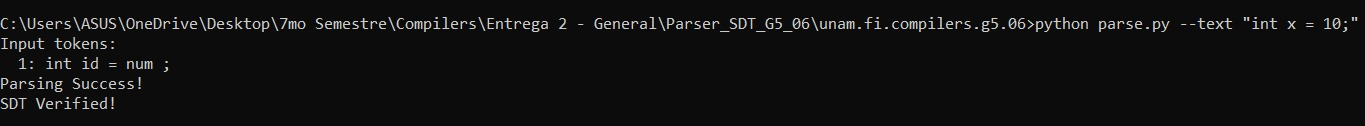
\includegraphics[width=\textwidth]{test_P1.jpeg}
    \caption{Execution of case P1: \texttt{int x = 10;}.}
\end{figure}

\subsection{P4: parsing error}

The input \texttt{int x 10;} has no \texttt{=} between the identifier and the number. The parse table has no entry for \texttt{Decl$'$} with the token \texttt{num}, so the parser reports the error. The SDT stage then reports the same error, because there is no complete parse tree to evaluate.

\begin{figure}[H]
    \centering
    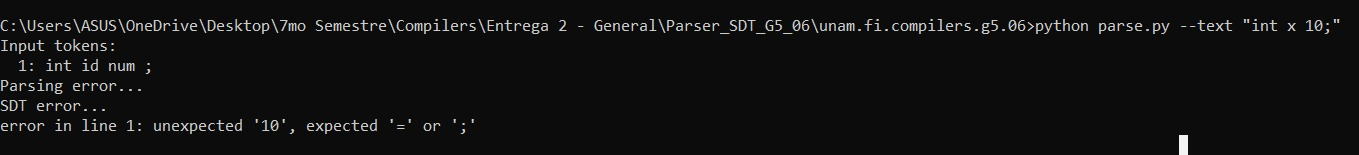
\includegraphics[width=\textwidth]{test_P4.jpeg}
    \caption{Execution of case P4: \texttt{int x 10;}.}
\end{figure}

\subsection{S1: implicit conversion allowed}

The input \texttt{float f = 10;} assigns an \texttt{int} to a \texttt{float} variable. This conversion is allowed by the type system, so both the parser and the SDT succeed.

\begin{figure}[H]
    \centering
    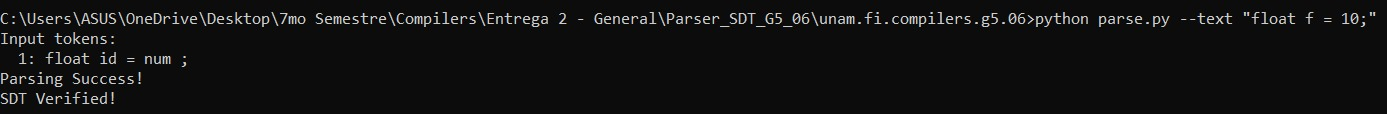
\includegraphics[width=\textwidth]{test_S1.jpeg}
    \caption{Execution of case S1: \texttt{float f = 10;}.}
\end{figure}

\subsection{S3: undeclared variable}

The input \texttt{int x = y + 1;} is syntactically correct, but \texttt{y} was never declared. Rule 24 reports the error once, and the error type propagates upward without producing additional messages.

\begin{figure}[H]
    \centering
    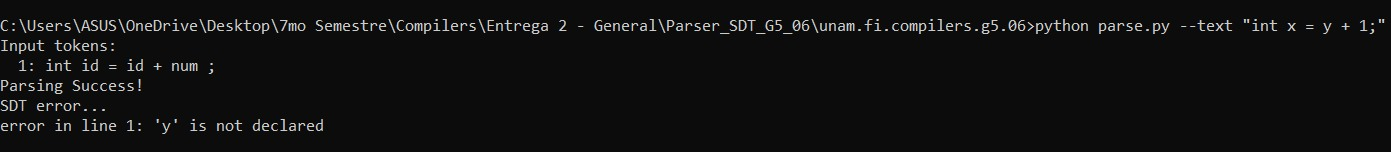
\includegraphics[width=\textwidth]{test_S3.jpeg}
    \caption{Execution of case S3: \texttt{int x = y + 1;}.}
\end{figure}

\subsection{S7: non-numeric operand}

The input \texttt{char c = \textquotesingle a\textquotesingle{} + 1;} is accepted by the parser, but the SDT rejects it because the operator \texttt{+} cannot be applied to a \texttt{char} and an \texttt{int} (rule 14).

\begin{figure}[H]
    \centering
    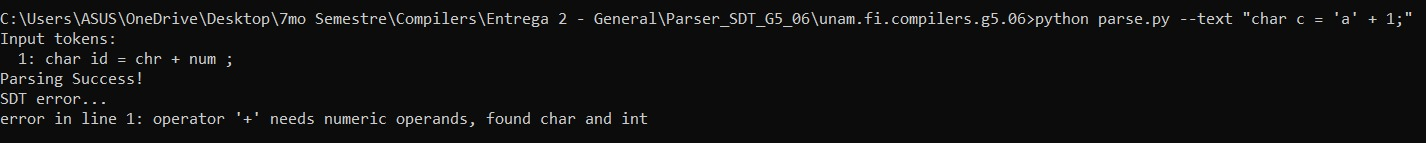
\includegraphics[width=\textwidth]{test_S7.jpeg}
    \caption{Execution of case S7: \texttt{char c = \textquotesingle a\textquotesingle{} + 1;}.}
\end{figure}

\section{Conclusions}
 
In this project we designed and implemented a top-down parser with a Syntax-Directed Translation (SDT) for a small C-like language with typed declarations, assignments, and arithmetic expressions. The grammar was transformed to remove left recursion and verified to be unambiguous and LL(1), using the FIRST and FOLLOW sets to build a parse table without conflicts. This guaranteed that the parser can decide each production with only one token of lookahead and without backtracking.\\
 
On top of the parser, the SDT adds the semantic checks that a grammar alone cannot express. Inherited attributes (such as the type that passes from \texttt{Type} to \texttt{Decl$'$}) and synthesized attributes (such as \texttt{Expr.type}) are evaluated over the parse tree, together with a symbol table that stores the type, size, and address of each variable. With the type system, the program rejects undeclared variables, repeated declarations, invalid operands, and incompatible assignments, while it allows the safe conversion from \texttt{int} to \texttt{float}.\\
 
The test cases confirm the separation between both stages. Inputs such as \texttt{int x 10;} fail in the parser, because of an empty cell in the parse table, while inputs such as \texttt{int x = y + 1;} and \texttt{char c = \textquotesingle a\textquotesingle{} + 1;} are syntactically correct and are rejected only by the SDT. Valid inputs such as \texttt{int x = 10;} and \texttt{float f = 10;} pass both stages. This shows that a correct syntax does not imply a correct meaning, and that both analyses are needed in a compiler.\\
 
Finally, working with a formal design (grammar, tables, attributes, and rules) before programming made the implementation more direct, and the error messages with the line number make the results easy to check. As future work, the language could be extended with more statements (conditionals and loops), and the SDT could generate intermediate code instead of only verifying types.\\

\section{References}

\begingroup
\setlength{\parindent}{-1.27cm}
\setlength{\leftskip}{1.27cm}
\setlength{\parskip}{0.4cm}

Aho, A. V., Lam, M. S., Sethi, R., \& Ullman, J. D. (2006). \textit{Compilers: Principles, techniques, and tools} (2nd ed.). Addison-Wesley.

Louden, K. C. (2004). \textit{Construcción de compiladores: Principios y práctica}. Thomson.

\endgroup

\end{document}